\chapter{Dokumentation af kode} \label{chap:kode_docs}
I dette kapitel vil funktioner i programmet blive forklaret.

\section{Loginsystem} \label{sec:login}
Formålet med et loginsystem er, at programmet kan holde styr på hvilken bruger der anvender systemet. 
Dette er vigtigt således reservationer placeres i det rigtige navn, og at brugeren kun har adgang til de rigtige funktioner. 
Eksempelvis skal et medlem af sejlklubben, ikke have adgang til at tilføje og fjerne brugere. 

Loginproceduren består fra brugeres synspunkt af at indtaste sit brugernavn og adgangskode, og trykke på login eller enter. 
Hvis brugeren har tastet rigtigt, vises deres en velkomstbesked og, afhængigt af brugerens privileger, får vedkommende adgang til de funktioner de har til rådighed.

Når loginet udføres af brugeren, oprettes der en forbindelse til databasen, hvorefter den tjekker hvorvidt de informationer, som er givet, stemmer overens med dens. 
Dog anvendes der en kryptografisk hashing algoritme. Dette er for at undgå, at folk med adgang til databasen kan aflæse brugernes adgangskoder.
Det er en præventiv beskyttelse mod hacking angreb.

\begin{wrapfigure}{l}{0.5\textwidth}
    \label{img:login_interface}
    \vspace{-20pt}
    \begin{center}
        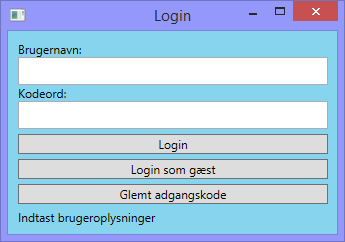
\includegraphics[width=0.48\textwidth]{Login_Window_Empty_Fields.png}
    \end{center}
    \vspace{-15pt}
    \caption{Login interface}
    \vspace{10pt}
\end{wrapfigure}
I programmet anvendes SHA-256, som returner en 256 bit hash (dvs. 32 bytes og 64 karakterer som en streng). 
Men dette ville være trivielt, at udskifte med en anden hashing algoritme, hvis der blev fundet en svaghed i SHA-256. 

Login interfacet (Figur \ref{img:login_interface}) giver også mulighed for at logge ind anonymt, som en gæst. 
Dette udføres ved at trykke på ``Login som gæst''-knappen. 
Login knappen (samt at trykke på ``Enter''/``Return''-knappen mens tekstfelterne er i fokus), udfører et login.
Samt giver brugeren adgang til et passende interface i hendhold til tabel \ref{tab:permissions}.


% LaTeX tabel som viser alle brugerniveauer og deres muligheder efter login.
% http://bit.ly/1kToHZ3 to edit raw table
\begin{table}
    \colorlet{shadecolor}{gray!40}
    \rowcolors{1}{white}{shadecolor}
    \begin{tabular}{l|llllll}
    ~                        & Gæst & Supportmedlem & Medlem & Elev & Underviser & Administrator \\ \hline
    Personlig forside        & ~    & ~             & \ding{51}     & \ding{51}    & \ding{51}          & \ding{51}             \\
    Se begivenheder          & \ding{51}    & \ding{51}             & \ding{51}      & \ding{51}    & \ding{51}          & \ding{51}             \\
    Tilmeld begivenheder     & ~    & \ding{51}             & \ding{51}      & \ding{51}    & \ding{51}          & \ding{51}             \\
    Opret begivenheder       & ~    & ~             & ~      & ~    & \ding{51}          & \ding{51}             \\
    Se sejlture              & \ding{51}    & \ding{51}             & \ding{51}      & \ding{51}    & \ding{51}          & \ding{51}             \\
    Opret sejltur            & ~    & ~             & \ding{51}      & \ding{51}    & \ding{51}          & \ding{51}             \\
    Se logbøger              & \ding{51}    & \ding{51}             & \ding{51}      & \ding{51}    & \ding{51}          & \ding{51}             \\
    Opret logbog             & ~    & ~             & \ding{51}      & \ding{51}    & \ding{51}          & \ding{51}             \\
    Svar på logbog           & ~    & ~             & ~      & ~    & ~          & \ding{51}             \\
    Se undervisningstimer    & ~    & ~             & ~      & \ding{51}    & \ding{51}          & \ding{51}             \\
    Opret undervisningstimer & ~    & ~             & ~      & ~    & \ding{51}          & \ding{51}             \\
    \end{tabular}
    \caption{Tabel over alle brugerniveauer og deres tilladte funktioner.}\label{tab:permissions}\fixme{Måske skal denne tabel lige laves lidt om, enten indholdet, eller hvordan det virker i programmet.}

\end{table}

\section{Primære brugergrænseflade}
Det primære vindue tilgåes via login vinduet, som er det der starter ved programstart, eller logud. 
Der findes 4 vinduer, forskellen mellem dem er hvilke tabs der er aktive. 
I hver tab findes der en funktionalitet, samlet set findes følgende tabs:
\begin{itemize}% Denne skulle måske relatere til tabel tab:permission
    \item Forside
    \item Undervisning
    \item Begivenheder
    \item Medlemmer
    \item Både
\end{itemize}

Via hver af disse tabs, vil der være adgang til programmet forskellige funktionaliteter.
Der er også en log ud knap, som bruges til at vende tilbage til loginvinduet, således en anden bruger kan anvende systemet.
Programmet er lavet til at køre i opløsningen 1024x720 pixels.
Denne opløsning er valgt for at understøtte alt fra bærbare, med opløsninger som 1366x768 pixels i et vindue, og op til FullHD (1920x1080 pixels) osv.
Programmet har et lyst farveskema, men farverne hvid og en lys blå som hovedfarver (\#87D4EE).


%\section{Klasser}
%\begin{minipage}[t]{1\linewidth}
%Set imagepath and scaling, imagepath set to start in images/UmlMini folder, just write filename and extension
%FBox added for outline on items
%\begin{wrapfigure}{l}{0.5\textwidth}
%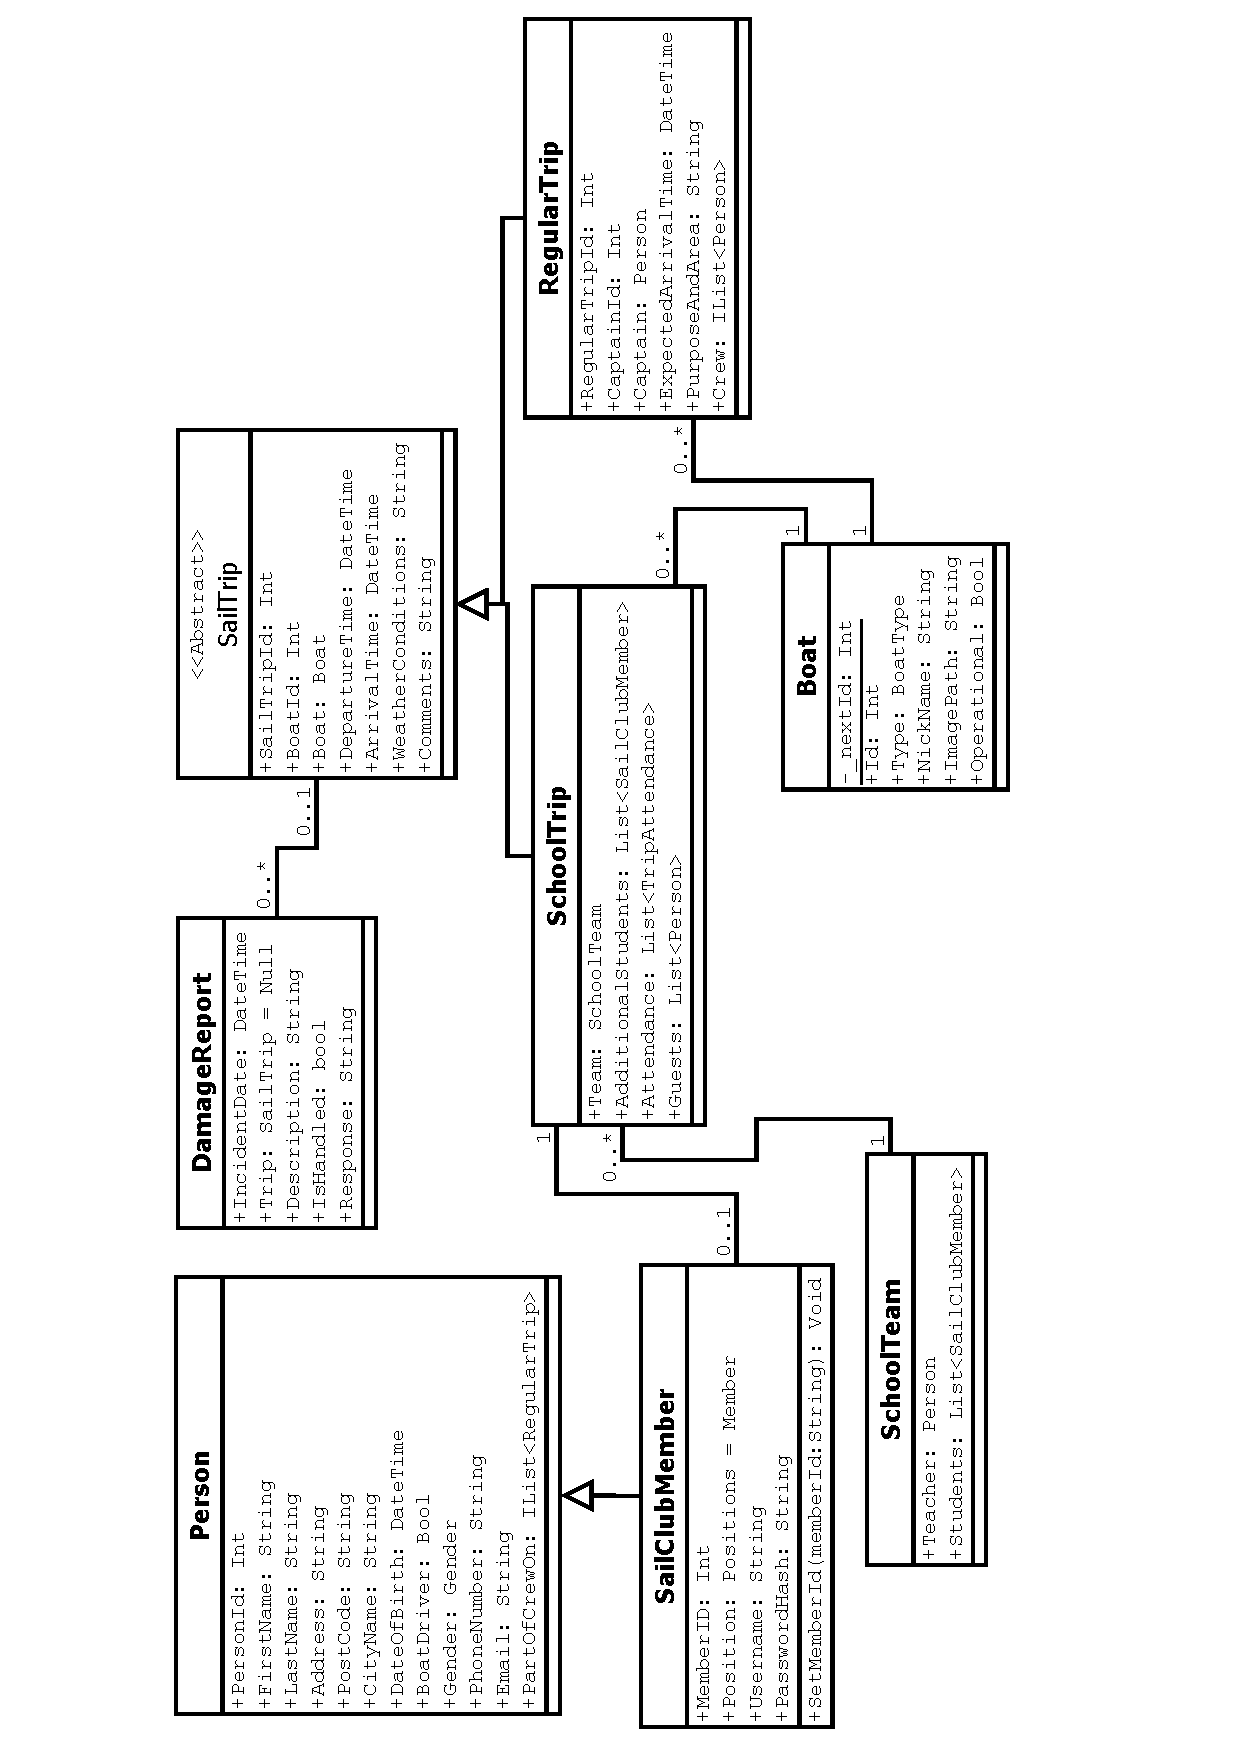
\includegraphics[scale=0.3]{UML.pdf}
%\end{wrapfigure}
%Brødtekst
%\end{minipage}

 